     %%%%%%%%%%%%%%%%%%%%
     %                  %
     %  capitolo5.tex   %
     %                  %
     %%%%%%%%%%%%%%%%%%%%

\chapter{Coupling to the gravitational field}
\noindent
In this chapter I will study the behavior of an $O(N)$ model coupled to a gravitational field.
For the conventions and formulas used in this chapter, see the Appendix D.



This matter-gravity system as a QFT can be consistent at quantum level only if it is ultraviolet complete and can be described by a finite number of physical parameters. 
In other words, if it is renormalizable in the most broader sense.
In is known that such models are typically non perturbatively renormalizable, but they still could be asymptotically safe at the non perturbative level.

Therefore we shall investigate this model with functional renormalization group techiques.



\section{FRG for gravity}
In this section I will expose some basic concepts necessary in order to extend the formalism of the functional renormalization group, 
developed in the previous chapters for a scalar field theory, to include a coupling with a dynamical spacetime metric. For this section
I will mainly follow \cite{reuter} and \cite{Percacci:2015wwa}.


In order to derive a functional integral formulation for a quantum theory of gravity, we need to give a precise meaning to a functional of the form:
\begin{equation}
 \int \mathcal{D}g_{\mu\nu} \e^{-S[g_{\mu\nu}] + \text{source terms}}
\end{equation}
where the bare action $S[g_{\mu\nu}]$ must be invariant under gauge tranformation, \emph{i.e.} under the transformation of the metric
under an infinitesimal diffeomorphism, that is given by:
\be
\label{gauge}
\delta_\epsilon g_{\mu\nu}=
\Lie_\epsilon g_{\mu\nu}
\equiv
\epsilon^\rho\partial_\rho g_{\mu\nu}
+g_{\mu\rho}\partial_\nu\epsilon^\rho
+g_{\nu\rho}\partial_\mu\epsilon^\rho\ .
\ee
where $\Lie_\epsilon$ is  the Lie derivative with respect the infinitesimal vector field $\epsilon$.


The most employed method in the literature is called the \emph{background field method}. 

Following this approach, the full metric have to be decomposed into a classical arbitrary (but fixed) background and the quantum fluctuation.


Some different decompositions have been investigated in the literature, our choice is to use 
an exponential parametrization:
\begin{equation} \label{decompo}
g_{\mu\nu}=\bg_{\mu\rho}(e^h)^\rho{}_\nu
\end{equation}
where $\bg_{\mu\rho}$ is a fixed but arbitrary background and $h$ is a two index tensor which encodes the quantum fluctuations \cite{Percacci:2015wwa}. We also assume the fluctuations to be small with respect to the background.

After this split, the functional integration measure $\mathcal{D} g_{\mu\nu}$ becomes $\mathcal{D} h_{\mu\nu}$.

If one uses the functional measure of a linear splitting ($\bar{g}_{\mu\nu} = {g}_{\mu\nu} + {h}_{\mu\nu})$, 
then one should take into account a Jacobian \cite{Percacci:2015wwa} which for our purposes, in the formalism considered, will not contribute.

Being this a gauge theory described by a redundant number of degrees of freedom, the path integral should be defined with care.
Usually one employs a gauge fixing condition and the Faddeev-Popov determinant, which depends on how  the gauge fixing conditionchanges with a gauge transformation. 
Such a determinant is usually written in terms of a functional integral over the \emph{ghost fields}.

%Now we need to state a gauge fixing condition, in order to apply the Faddeev-Popov trick \cite{reuter46}.
We shall define the ``quantum'' gauge transformation as a special gauge transformation that reproduces \eqref{gauge} when the background is kept
fixed:
\begin{equation}
 \mathcal{L}_\epsilon g_{\mu\nu} = \bar{g}_{\mu\rho}\mathcal{L}_\epsilon (e^h)^\rho{}_\nu
\end{equation}

So the gauge tranformation is given, for small $h$, by the following relation:
\be
\delta^{(Q)}_\epsilon h^\mu{}_\nu=
\bnabla^\mu\epsilon_\nu+\bnabla_\nu\epsilon^\mu
+\Lie_\epsilon h^\mu{}_\nu
+[\Lie_\epsilon\bar g,h]^\mu{}_\nu
+O(\epsilon h^2)\ .
\ee
Once fixed the gauge , we can define the
running Schwinger functional by the following expression:
\begin{equation*}
 \exp \{W_k [J^{\mu\nu}, \sigma^\tau, \bar{\sigma}_\rho, \bg_{\mu\rho}]\} = \int \mathcal{D}h_{\mu\nu} \mathcal{D}C^\rho\mathcal{D}\bar{C}_\tau \mu_{GF} \exp \Big\{-S[{g}_{\mu\nu} ] - 
\end{equation*}
\begin{equation}\label{Wgravi}
 -S_{gh}[{g}_{\mu\nu}, C^\rho,\bar{C}_\tau] - S_{\text{source}} -\Delta_kS\Big\}
\end{equation}

where I have indicated with $C^\rho$ and $\bar{C}_\tau$ the Faddeev-Popov ghosts, $J^{\mu\nu}, \sigma^\tau$,  $\bar{\sigma}_\rho$ are the sources coupled to $h_{\mu\nu}$, $C^\rho$, $\bar{C}_\tau$ respectively and
$\mu_{GF}$ is the measure related to the gauge fixing.

As we can see , the action is given by the sum of several terms:
\begin{enumerate}
 \item the Einstein Hilbert action with a cosmological constant $\Lambda$:$$S[{g}_{\mu\nu}] = \frac{1}{16\pi G}\int d^D x \sqrt{g} (2\Lambda_C - R)$$ 
 \item the ghosts action, $S_{gh}[\bar{g}_{\mu\nu}, h_{\mu\nu}, C^\rho,\bar{C}_\tau]$, which is related to the Faddeev-Popov determinant associated to the gauge fixing condition;
 \item the source term:  $$ S_{\text{source}} = -\int d^D x \sqrt{\bar{g}} \big(J^{\mu\nu}h_{\mu\nu}+C^\rho\bar{\sigma}_\rho +\sigma^\tau\bar{C}_\tau\big)$$
 \item the regulator term, which encodes the scale dependence: $$\Delta_k S = \frac{1}{2} \int  d^D x \sqrt{\bar{g}}h_{\alpha\beta}\big(R_k^{gr}[\bar{g}]\big)^{\alpha\beta\gamma\delta}h_{\gamma\delta} + \sqrt{2} \int  d^D x \sqrt{\bar{g}}\bar{C}_\mu R_k^{gh}[\bar g]C^\mu$$
\end{enumerate}
From equation \eqref{Wgravi} we can define the classical fields:
\begin{equation}
 \bar{h}_{\mu\nu}=\frac{1}{\sqrt{\bar{g}}}\frac{\delta W_k}{\delta J^{\mu\nu}}\ , \ \ \ \ \ c^\mu=\frac{1}{\sqrt{\bar{g}}}\frac{\delta W_k}{\delta \bar{\sigma}_\mu}\ , \ \ \ \ \ \bar{c}_\mu=\frac{1}{\sqrt{\bar{g}}}\frac{\delta W_k}{\delta \sigma^\mu}
\end{equation}
Now, in analogy to what I have exposed in chapter 2 (see eq.\eqref{convessa}), we can define the effective average action as the modified 
Legendre transform of $W_k$:
\begin{equation}
 \Gamma_k[\bar h, c, \bar c; \bar g] = W_k[J, \sigma, \bar \sigma; \bar g] - \int d^D x \sqrt{\bar{g}} \big(J^{\mu\nu}\bar h_{\mu\nu} + c^\mu\bar \sigma_{\mu} + \bar c_\mu\sigma^\mu \big) - \Delta S_k
\end{equation}
Now, repeating the same procedure exposed in chapter 2 with  few differences, we come to the following generalization of the Wetterich equation:
\begin{equation}\label{supertraccia}
  \dot{\Gamma}_k = \frac{1}{2}\Tr\left\{\left[\left(\Gamma_k^{(2)}\right)_{\bar{h}\bar{h}} + R_k^{gr}\right]^{-1}\partial_tR_k^{gr} \right\} - \Tr\left\{\left[\left(\Gamma_k^{(2)}\right)_{c\bar{c}} + R_k^{gh} \right]^{-1}\partial_t R_k^{gh} \right\}
\end{equation}
where I have used the shorthand notations:
\begin{equation}
 \left(\Gamma_k^{(2)}\right)_{\bar{h}\bar{h}} = \frac{1}{\sqrt{ \bar g}} \frac{\delta}{\delta h_{\alpha \beta}}\left(\frac{1}{\sqrt{ \bar g}} \frac{\delta \Gamma_k}{\delta h_{\mu\nu}}\right)
\end{equation}
\begin{equation}
 \left(\Gamma_k^{(2)}\right)_{c\bar{c}} = \frac{1}{\sqrt{ \bar g}} \frac{\delta}{\delta c_\mu}\left(\frac{1}{\sqrt{ \bar g}} \frac{\delta \Gamma_k}{\delta \bar c_\nu}\right)
\end{equation}

Equation \eqref{supertraccia} can also be rewritten in the more compact notation:
\begin{equation}\label{superwetterich}
  \dot{\Gamma}_k = \frac{1}{2}\STr\left\{\left[\Gamma_k^{(2)}+ R_k\right]^{-1}\partial_tR_k\right\}
\end{equation}
where $\STr\{\dots\}$ indicates the supertrace operation.


\section{Derivation of the fixed point equations}
In the foollowing we shall apply this formalism in the presence of an interacting $O(N)$ multiplet of scalar fields.

I assume the effective average action of the model can be truncated in the following form:
\begin{equation}
\label{ONaction5}
\Gamma_k [\phi, g] = \int {d}^Dx\sqrt{g}\left(U(\rho)+\frac{1}{2}\bg^{\mu\nu} \partial_\mu\phi^a \partial_\nu \phi_a-F(\rho)R\right)
\end{equation}
Where I have indicated with $S_{GF}$ and $S_{gh}$ the gauge fixing and the ghost terms respectively.

In the limit of a constant classical field $\phi$ we recover the usual Einstein-Hilbert action, while in the limit of a 
vanishing gravitational field (that means, in an Euclidean spacetime, $g_{\mu\nu} = \delta_{\mu\nu}$) we recover the well
known linear $O(N)$ model in the LPA.

I will employ the background-fluctuation split for the fields on the $O(N)$ field, so we have:
\begin{equation}
 \phi^i(x) = \bar{\phi}^i + \delta \phi^i(x), \ \ \ \ \ \ \ \bar{\rho} = \frac{\bar{\phi}^i\bar{\phi}_i}{2}
\end{equation}
For what concerns the metric, I will use the following parametrization:
\be
\label{decomp}
g_{\mu\nu}=\bg_{\mu\rho}(e^h)^\rho{}_\nu
\ee
Defining $h_{\mu\nu}=\bg_{\mu\rho}h^\rho{}_\nu$, we have:
\bea
g_{\mu\nu}&=&\bg_{\mu\nu}+h_{\mu\nu}
+\frac{1}{2}h_{\mu\lambda}h^\lambda{}_\nu+\ldots
\\
g^{\mu\nu}&=&\bg^{\mu\nu}-h^{\mu\nu}
+\frac{1}{2}h^{\mu\lambda}h_\lambda{}^\nu+\ldots
\eea


In order to obtain the Hessian of the model, I have expanded the effective average action \eqref{ONaction5} up to the second order in the fluctuations.

It results to be the sum of two pieces, one quadratic in the scalar field fluctuation:
\be
\!\frac{1}{2}\! \int {d}^D x \sqrt{\bg} 
\,\delta\phi^a \!\Big\{ \left[-\nabla^2\!+\!U'(\brho) \!-\!\bR F'(\brho) \right] \widehat{\phi}^{a}\widehat{\phi}^{b} +
\ee
\begin{equation}
 +\left[ -\nabla^2\!+\!U'(\brho)\!+\!2\brho U''(\brho)\!-\!\bR \left(F'(\brho)+2\brho F''(\brho)\right) \right] \!(\delta^{ab} - \widehat{\phi}^{a}\widehat{\phi}^{b})\Big\} \delta\phi^b
\end{equation}
and another which mixes scalar field fluctuations with metric scalar fluctuations:
\be\label{longmetrica}
 \int {d}^D x \sqrt{\bg} \, \delta\phi^a  \bphi^b \left[ \frac{h}{2} U'(\brho)
-F'(\brho)  \left( \bnabla_\mu  \bnabla_\nu h^{\mu\nu}-\bnabla^2 h -\bR_{\mu\nu} h^{\mu\nu} +\frac{\bR}{2} h \right) \right]\widehat{\phi}^{a}\widehat{\phi}^{b}
\Bigr\}
\ee
where I recall that $\widehat{\phi}^{i}$ is defined as:
 $$\widehat{\phi}_{a} = \frac{\bar{\phi}_{a}}{\sqrt{2\bar{\rho}}}$$
so, $(\delta^{ab} - \widehat{\phi}^{a}\widehat{\phi}^{b})$ and $\widehat{\phi}^{a}\widehat{\phi}^{b}$ are the projectors on the longitudinal ($P_L^{ab}$, in the following) and on the transverse ($P_T^{ab}$) directions respectively.

It's easy to see, from equation \eqref{longmetrica}, that only the longitudinal scalar fluctuations mix in the Hessian with the scalar fluctuations of the metric.

This last term can be rewritten in a more useful way after the York decomposition of the traceless part of $h_{\mu\nu}$.
Doing that and rescaling in terms of $\sigma'$ and $h=2d\omega$ we obtain:
\begin{equation*}
- \int {d}^D x \sqrt{\bg} \, \delta\phi_a P_L^{ab} \bphi^b \left\{ F'(\brho)  \frac{D-1}{D} 
\left[ \sqrt{ -\bnabla^2 \left(-\bnabla^2 -\frac{\bR}{D-1}\right) } \sigma' +\left(-\bnabla^2 +\frac{(D-2) \bR}{2(D-1)} \right) h \right]- \frac{U'(\brho)}{2} h \right\}
\end{equation*}
Now we can use the gauge invariant variable $s=h-\bnabla^2 \sigma$. In terms of the rescaled field we have the relations:
\be
\sigma=\frac{1}{\sqrt{(-\bnabla^2)\left(-\bnabla^2-\frac{R}{D-1}\right)}}\sigma'\,, \quad s=h+\frac{\sqrt{-\bnabla^2}}{\sqrt{-\bnabla^2-\frac{R}{D-1}}}\sigma' \,,\quad 
\sigma'=\frac{\sqrt{-\bnabla^2-\frac{R}{D-1}}}{\sqrt{-\bnabla^2}}(s-h)
\ee
The last term can be written as
\be
 \int {d}^D x \sqrt{\bg} \, \delta\phi^a P_L^{ab} \bphi^b  \left[ - \frac{D-1}{D} F'(\brho)
  \left(-\bnabla^2 -\frac{\bR}{D-1}\right) s +\frac{U'(\brho) - F'(\brho) \bR}{2} h \right]
\ee
The gravitational hessian can be transformed into:
\begin{equation*}
\label{hessian2}
\frac{1}{2} \int {d}^D x\sqrt{\bg}F(\brho) \Biggl[
\frac{1}{2}\tth_{\mu\nu}\left(\!-\bnabla^2\!+\!\frac{2\bR}{D(D-1)}\right)\tth^{\mu\nu}
\!- \frac{(D\!-\!1)(D\!-\!2)}{2d^2} s \left(-\bnabla^2\!-\!\frac{\bR}{D-1}\right) s
- \frac{D\!-\!2}{4d} \bR \,h^2\Biggr]
\end{equation*}

At this point one can make a $P_L \delta\phi$ dependent shift in the variable s to complete the $s$-$P_L \delta\phi$ square in the Hessian:
\be
s'=s+\frac{2D}{D-2}\frac{F'(\brho)}{F(\brho)} \bphi^a  \left(-\bnabla^2 -\frac{\bR}{D-1}\right) \delta\phi^a \,.
\ee
Then the full hessian can be written as:
\small{
\bea
\label{fullhessian}
&&\frac{1}{2} \int {d}^D x\sqrt{\bg}\Biggl\{ F(\brho) \Biggl[
\frac{1}{2}\tth_{\mu\nu}\left(\!-\bnabla^2\!+\!\frac{2\bR}{D(D-1)}\right)\tth^{\mu\nu}
\!- \frac{(D\!-\!1)(D\!-\!2)}{2D^2} s' \left(-\bnabla^2\!-\!\frac{\bR}{D-1}\right) s'
\Biggr]
\nonumber\\
&&
 \qquad\qquad
 - \frac{D\!-\!2}{4D}  F(\brho) \bR\,h^2+\delta\phi^a \bphi^a\Bigl[{U'(\brho) - F'(\brho) \bR}\Bigr] h+
\nonumber\\
&&
\qquad\qquad
+\delta\phi^a  \left[ -\nabla^2\!+\!U'(\brho)\!+\!2\brho U''(\brho)\!-\!\bR \left(F'(\brho)+2\brho F''(\brho)\right) +\right.
\nonumber\\
&&
+ \left. \frac{4\brho (D-1)}{D-2} \frac{(F'(\brho))^2}{F(\brho)}  \left(-\bnabla^2 -\frac{\bR}{D-1}\right) \right] +
\!P_L^{ab} \delta\phi^b
\nonumber\\
&&
\qquad\qquad
+\delta\phi^a \Bigl[-\nabla^2\!+\!U'(\brho) \!-\! F'(\brho)\bR\ \Bigr] P_\perp^{ab}  \delta\phi^b
\Biggr\}
\eea
}
We can now employ the gauge fixing $\xi=0$ and $h=0$ (unimodular gauge).

Regarding the regulator function, $\mathcal{R}_k $, it is a matrix valued function as $\Gamma^{(2)}$. A convenient definition for it
is by the relation:
\begin{equation}
  \Gamma_k^{(2)} (\bar \nabla^2) + \mathcal{R}_k(-\bar \nabla^2) = \Gamma_k^{(2)} (P_k(-\bar \nabla^2))
\end{equation}
where the function I have defined the function $P_k(-\bar \nabla^2)$ in the following way:
$$P_k(-\bar \nabla^2)= -\bar \nabla^2 + R_k(-\bar \nabla^2)$$ 
and $R_k$ is a single valued function that must satisfy the relations \eqref{relazione1}, \eqref{relazione2} and \eqref{relazione3}, that we choose to have the form of an optimized Litim regulator:
\begin{equation}
 R_k(- \bar \nabla^2) = (k^2 - (- \bar \nabla^2))\theta(k^2 - (- \bar \nabla^2)) 
\end{equation}
The last step is to define a method to evaluate the trace in \eqref{superwetterich}. In the literature this is usually done using the \emph{heat kernel technique},
whose details are not exposed in this thesis, for details see, for example, \cite{heat}.

Now we have all the elements to compute the traces and, consequently, to obtain the flow equations for the dimensionless $u$ and $f$.

At the fixed point, for $D=3$, we obtain the following equations for the scaling solution:

\bea
\label{eqFPd3}
0&=&-3 u(\rho )+\rho  u'(\rho )+\frac{N-1}{6 \pi ^2 \left(u'(\rho )+1\right)}-\frac{2 \rho  f'(\rho )+3 f(\rho )}{30 \pi ^2 f(\rho )}
\nonumber\\
&&
+\frac{f(\rho ) \left(12 \rho  u''(\rho )+6 u'(\rho )+11\right)-\rho  f'(\rho ) \left(16 \rho  f''(\rho )-80 f'(\rho )+2 \rho  u''(\rho )+u'(\rho
   )+1\right)}{30 \pi ^2 \left(8 \rho  f'(\rho )^2+f(\rho ) \left(2 \rho  u''(\rho )+u'(\rho )+1\right)\right)} \,.
\nonumber\\
0&=&-f(\rho )+\rho  f'(\rho )-\frac{(N-1) f'(\rho )}{6 \pi ^2 \left(u'(\rho )+1\right)^2}-\frac{N-1}{24 \pi ^2 \left(u'(\rho )+1\right)}+\frac{101}{120 \pi ^2}-\frac{29 \rho  f'(\rho )}{180 \pi ^2 f(\rho )}
\nonumber\\
&&
+\frac{\rho  f'(\rho ) \left(16 \rho  f''(\rho )-48 f'(\rho )+2 \rho  u''(\rho )+u'(\rho )+1\right)-f(\rho ) \left(8 \rho  u''(\rho )+4 u'(\rho
   )+7\right)}{72 \pi ^2 \left(8 \rho  f'(\rho )^2+f(\rho ) \left(2 \rho  u''(\rho )+u'(\rho )+1\right)\right)}
  \nonumber\\
  &&
  -\frac{\left(8 \rho ^2 f'(\rho )^3-16 \rho  f(\rho ) f'(\rho ) \left(\rho  f''(\rho )-2 f'(\rho )\right)+5 f(\rho )^2\right) \left(4 \rho  f'(\rho
   )^2+f(\rho ) \left(2 \rho  f''(\rho )+f'(\rho )\right)\right)}{30 \pi ^2 f(\rho ) \left(8 \rho  f'(\rho )^2+f(\rho ) \left(2 \rho  u''(\rho
   )+u'(\rho )+1\right)\right)^2}\,.
   \nonumber\\
  \eea


\section{Scaling solutions for D=3}
\subsection{Analytical solution for arbitrary N}
Two of the solutions of the system of the fixed point equations \eqref{eqFPd3} can be found analitically, making some ansatz on the 
functional form of $u(\rho)$ and $f(\rho)$. 

The first one is a configuration in which the effective potential $u(\rho)$ and $f(\rho)$ are both constant, which is also called \emph{Gaussian Matter fixed point}\cite{vacca24}:
\begin{equation}
\left\{
\begin{array}{l}
u (\rho) = u_0\\ \ \\
f (\rho) = f_0
\end{array}
\right.
\end{equation}
Indeed, substituting this conditions in the \eqref{eqFPd3} we find the solutions:
\begin{equation}
\left\{
\begin{array}{l}
u_0 = \frac{5 N+3}{90 \pi ^2}\\ \ \\
f_0 = \frac{283-15 N}{360 \pi ^2}
\end{array}
\right.
\end{equation}
in order to obtain a coherent physical picture of the gravity as an attractive interaction (\emph{i.e.} a positive Newton constant), both $u_0$ and $f_0$ must be positive. 
So the physical acceptability of this fixed point solution leads to the following condition on $N$:
\begin{equation}
 N <\frac{283}{15} \approx 18,8667
\end{equation}
The second one is a configuration of a nonminimal coupling with the gravitational feld, of the following form:
\begin{equation}
\left\{
\begin{array}{l}
u (\rho) = u_0\\ \ \\
f(\rho) =  f_1\rho
\end{array}
\right.
\end{equation}
that admits the solutions:
\begin{equation}\label{nonmatter}
\left\{
\begin{array}{l}
u_0 = 	\frac{N}{18 \pi ^2}		\\ \ \\
f_1 = \frac{80 - 9N \pm \sqrt{9 N^2-264 n+5296}}{48 (N-1)}
\end{array}
\right.
\end{equation}
but only the one with the plus sign can be positive, leading to the following constraint on $N$:
\begin{equation}
 1 < N < \frac{46}{3} \approx 15,3333
\end{equation}
Linearizing the flow equations in the neighborhood of a fixed point, one can evaluate the critical
exponents of the model. For example, the linearized flow equations  near the solution \eqref{nonmatter} reads, for any of the
allowed values of $N$:

$$0 =36 \left(\frac{1}{15N}-\frac{1}{283}\right) \rho  \delta f'(\rho )+\lambda  \left(\frac{36}{283}-\frac{12}{5 N}\right) \delta f(\rho) + $$
$$+\frac{(283-15 N)^2 \rho \delta u''(\rho )}{12735 \pi ^2 N}-\frac{(283-15 N)^2 \left(6 \pi ^2 \rho -1\right) \delta u'(\rho )}{25470 \pi^2 N}+\frac{(\lambda +3) (283-15 N)^2 \delta u(\rho )}{4245 N}$$

that is the $\delta u(\rho) $ flow equation, and:

$$0=\frac{(283-15N)^2 \rho\delta f''(\rho )}{12735 \pi ^2 N}+\frac{\left(\frac{1}{15 N}-\frac{1}{283}\right) \left(15 N \left(6 \pi ^2 \rho -1\right)-1380 \pi ^2 \rho +283\right) \delta f'(\rho )}{6 \pi ^2}+$$
$$+\left(\frac{1}{283}-\frac{1}{15 N}\right) \delta f(\rho ) (-230 \lambda +15 (\lambda +1) N-283)-\frac{(283-15 N)^2 \rho  \delta u''(\rho )}{50940 \pi ^2 N}-\frac{(283-15 N)^2 \delta u'(\rho )}{101880 \pi ^2 N}$$

for $\delta f(\rho)$.
\begin{comment}
\subsection{The $O(2)$ model: critical exponents for the Gaussian Matter fixed point}


As we have seen in the previous section, two of the fixed points of the model can be derived analytically, 
if we have putted some constraints on the allowed $N$. That is due to the requiring of an attractive gravitational interaction (or, in other words, 
of an always positive running coupling constant). The scalar $O(1)$ model, in which the only admitted analytical solution is the Gaussian
Matter fixed point, has been studied in \cite{Percacci:2015wwa}. 

Now I want to study the $O(2)$ model in the vicinity of the Gaussian Matter fixed point:

\begin{equation}
\left\{
\begin{array}{l}
u_0 = \frac{13}{90 \pi^2} \approx 0.0146353 \\ \ \\
f_0 = \frac{253}{360 \pi ^2} \approx 0.0712063
\end{array}
\right.
\end{equation}
deriving its critical exponents.

In order to linearize the flow equations, it's useful to perform the following change of variable, defining $\phi = \sqrt{2\rho}$.

\end{comment}
%%%%%%%%%%%%%%%%%%%%%%%%%%%%%%
\subsection{Numerical search for non trivial fixed points}
%%%%%%%%%%%%%%%%%%%%%%%%%%%%%%
The next step is to look for other non trivial fixed points, which can  be seen as a gravitational deformation of the Wilson Fisher fixed point of the Ising universality class when gravitational interactions are turned off. 
The method used is numerical, based on a \emph{shooting method}. 

We find very useful to start with an investigation of the evolution of the system non linear differential equations from the origin.
Since the differential equations have a fixed singularity at $\rho=0$ there is a constraint for solutions to be defined at the origin which lowers the number of parameters from $4$ to $2$.
We shall write the Cauchy problem as a function of $\sigma_1=u'(0)$ and $\sigma_2=f'(0)$ and study the outcome of the numerical evolution on varying such parameters.
We shall see that generically the numerical evolution stops when a singularity is reached. This is due to the fact that for generic initial conditions the non linear differential problem does not admit a global solution.
But there is a finite set of values for the parameters such that global solutions do exists. Two of such solutions have been already found analytically.
Our task is to see if there are other global solutions. In $D=3$ for at least some values of $N$ we expect them to exist.
If a global solution does exists, we expect that starting with initial conditions close enough one sees that the alghoritm, which evolves the numerical solution from the origin, stops at larger values of $\rho=\bar\rho$, 
which can be increased tuning the parameters encoding the initial conditions.
Therefore in our case we study numerically the function $\bar\rho(\sigma_1,\sigma_2)$ and by plotting such a function we should see a spike in correspondece of a possible global solution.

Numerically we shall study the numerical problem for $\rho\ge\epsilon$ for $\epsilon \to 0$.
The Cauchy problem is defined as:
\small{
\begin{eqnarray}
&{}& u'(\epsilon)=\sigma_1 \quad f'(\epsilon)=\sigma_2 \nonumber\\
&{}&u(\epsilon)=\frac{5 N+3 \sigma_1+3}{90 \pi ^2 (\sigma_1+1)}\nonumber\\
&{}&+\frac{\epsilon  \left(12 \sigma_2 (\sigma_1 (5 N+3 \sigma_1+6)+3)+\sigma_1 (\sigma_1+1) (15 N-283 (\sigma_1+1))
+96 (1-4 \sigma_1) \sigma_2^2\right)}{45 N (\sigma_1+4 \sigma_2+1)-849 (\sigma_1+1)^2}
\nonumber\\
&{}&f(\epsilon)=
\frac{283 (\sigma_1+1)^2-15 N (\sigma_1+4 \sigma_2+1)}{360 \pi ^2 (\sigma_1+1)^2}+
\end{eqnarray}
\begin{equation}
 +\frac{\sigma_2 \epsilon  \left(-20 (\sigma_1+1) \sigma_2 (3 N+4 \sigma_1+10)+5 (\sigma_1+1)^2 (46 (\sigma_1+1)-3 N)+192 (3-2 \sigma_1) \sigma_2^2\right)}{(\sigma_1+1) \left(283 (\sigma_1+1)^2-15 N (\sigma_1+4 \sigma_1+1)\right)} 
\end{equation}
}
   
where the condition on $u(\epsilon)$ and $f(\epsilon)$ have been determined to first order in $\epsilon$ by imposing that the differential equations should be satisfied.

We have then analyzed numerically $\bar\rho(\sigma_1,\sigma_2)$ for some values of $N$.
We report in Fig.\ref{fig:1}, \ref{fig:2}, \ref{fig:3}, \ref{fig:4} and \ref{fig:5} the cases for $N=1,\ 1.5,\ 2$.



\begin{figure}
\begin{center}
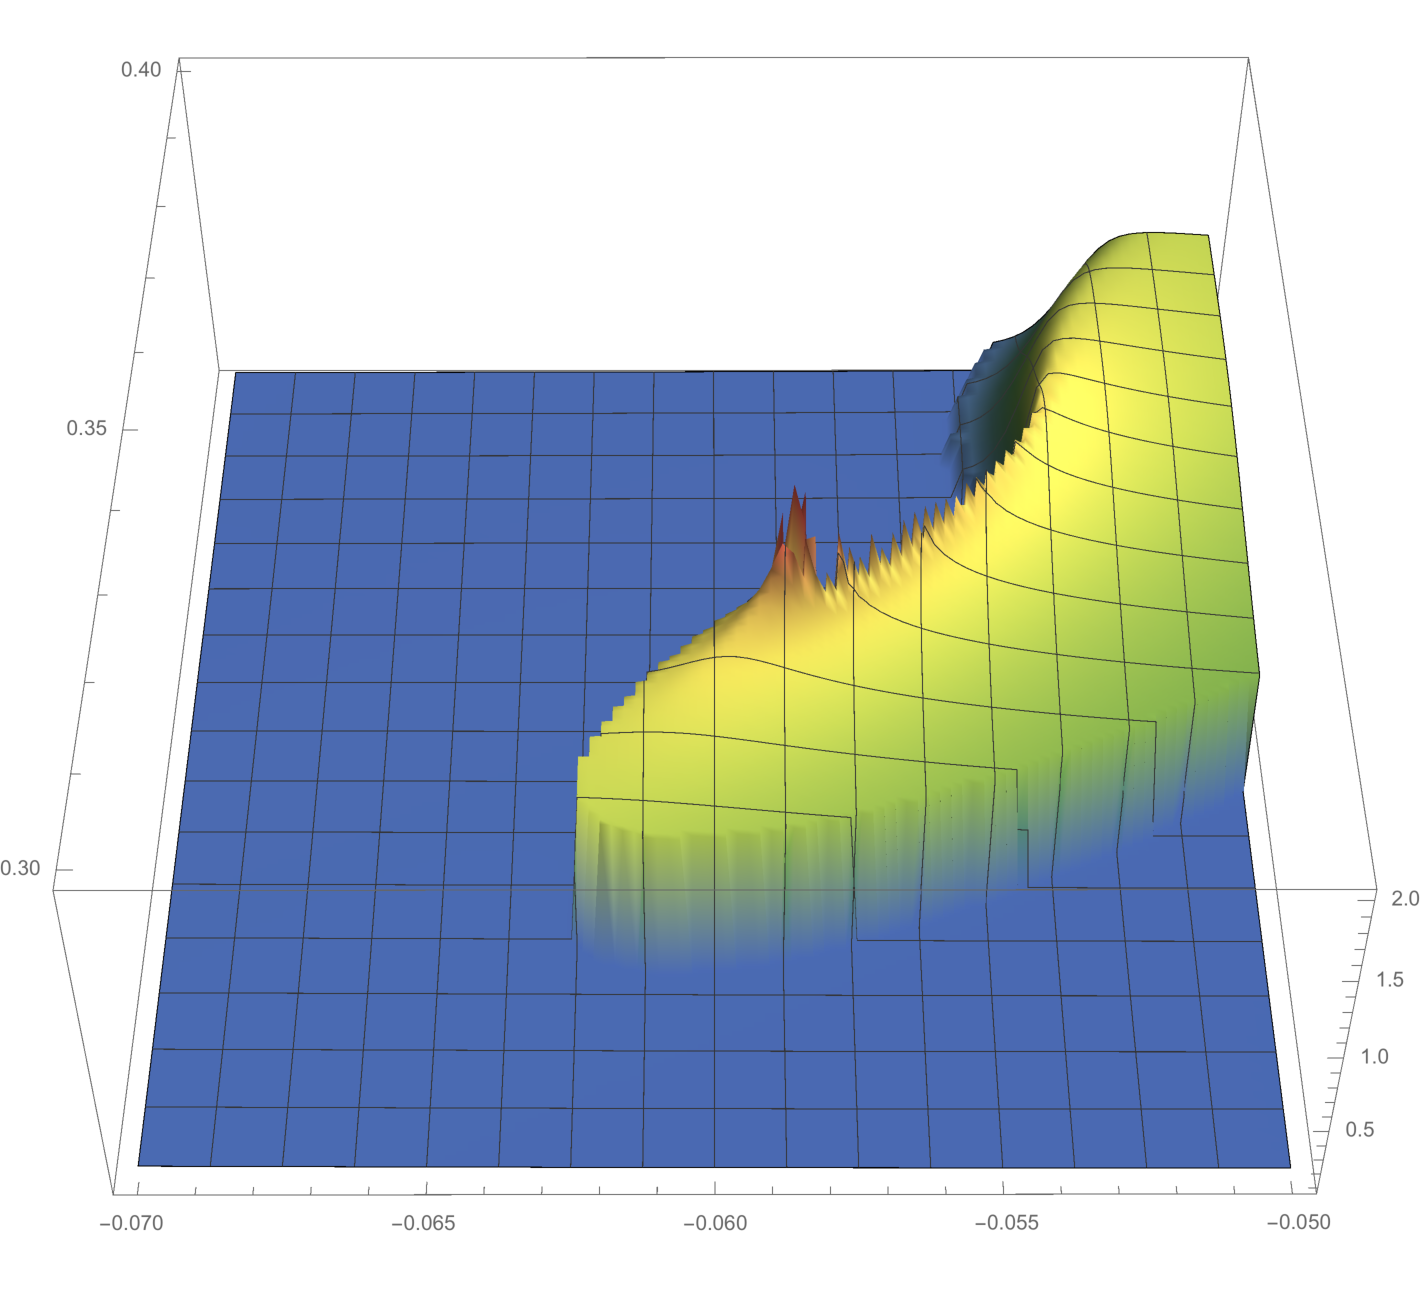
\includegraphics[scale=0.5]{Immagini/spiked3N1.pdf}
\caption{The case $N=1$. The peak is located at $(-0.0585, 0.344)$.}
\label{fig:3}
\end{center}
\end{figure}


\begin{figure}
\begin{center}
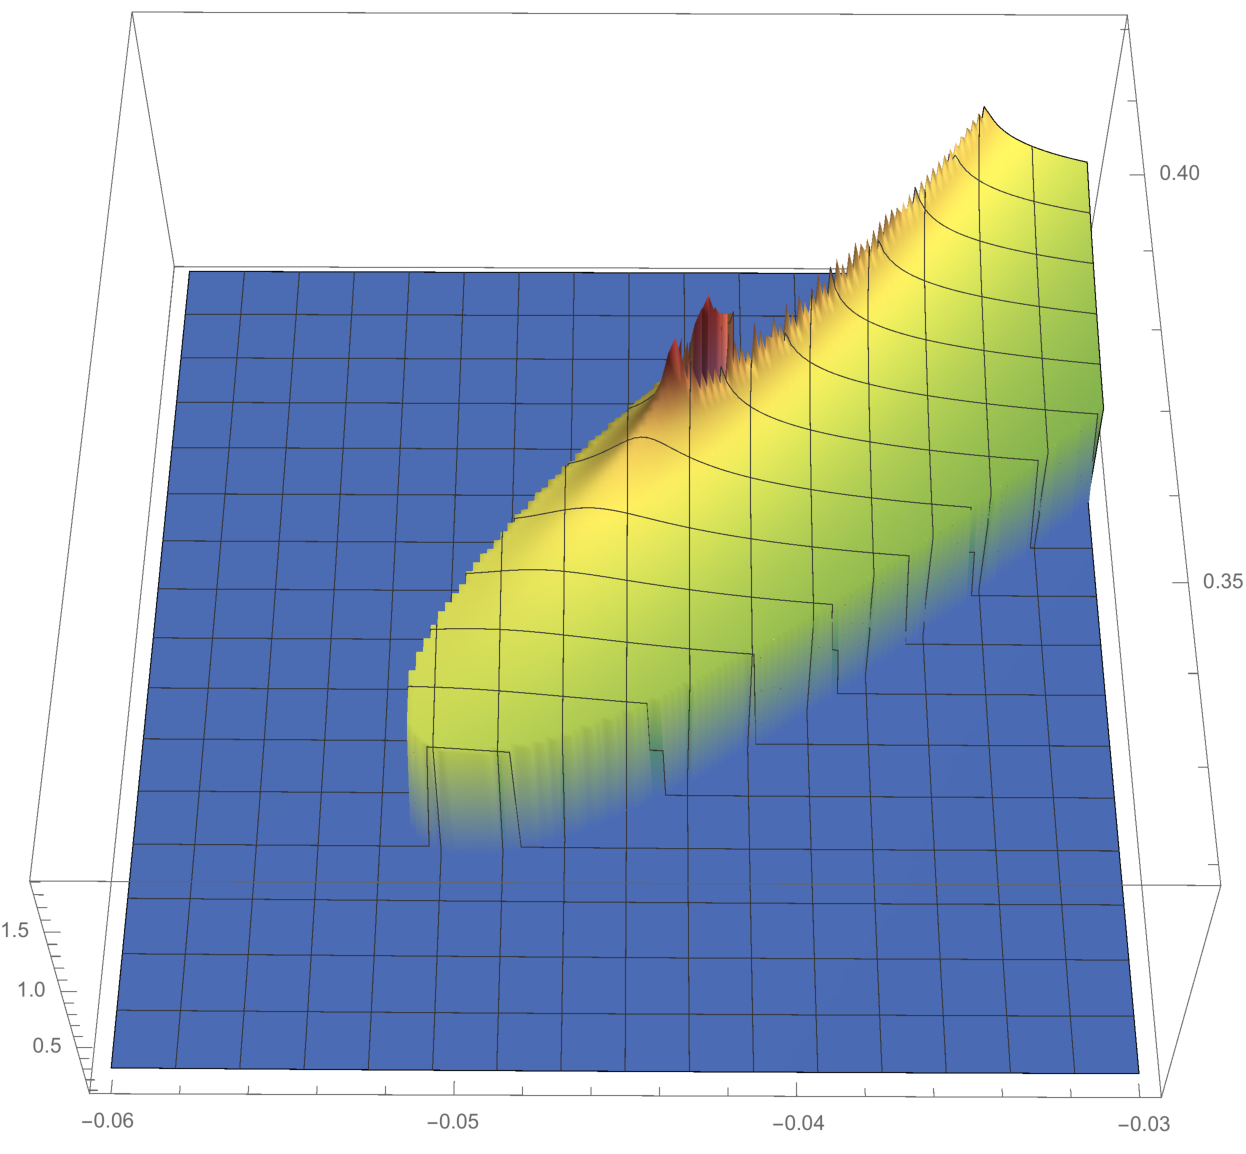
\includegraphics[scale=0.5]{Immagini/spiked3N1p5.pdf}
\caption{Plot of the function $\bar \rho (\sigma_1, \sigma_2)$ for N = 3/2. The peak results to be located at $(-0.0425, 0.385)$}
\label{fig:1}
\end{center}
\end{figure}


\begin{figure}
\begin{center}
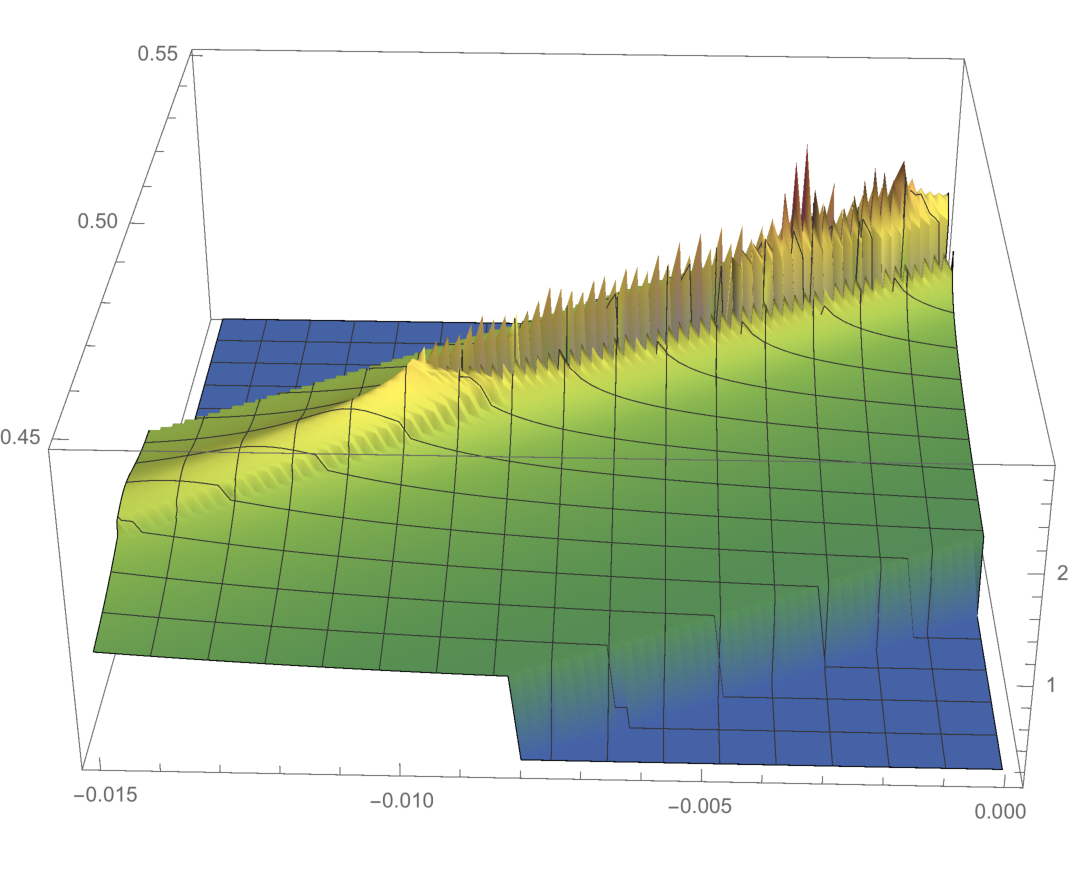
\includegraphics[scale=0.5]{Immagini/spiked3N2front.pdf}
\caption{Plot of the function $\bar \rho (\sigma_1, \sigma_2)$ for N = 2. It looks like there are two peaks, one close to the other.}
\label{fig:2}
\end{center}
\end{figure}


\begin{figure}
\begin{center}
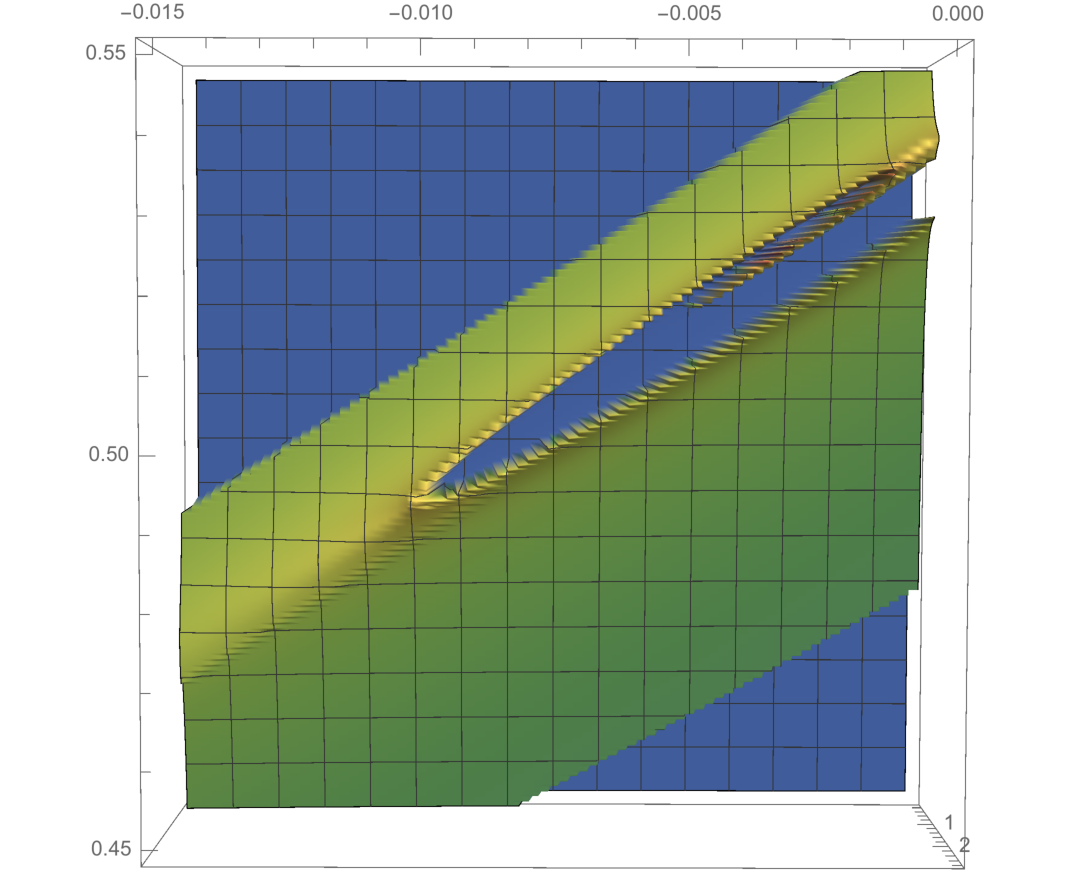
\includegraphics[scale=0.5]{Immagini/spiked3N2top.pdf}
\caption{A top view of the two peaks in the case $N=2$. The highest peak is located at (-0.0029, 0.5260)}
\label{fig:4}
\end{center}
\end{figure}



\begin{figure}
\begin{center}
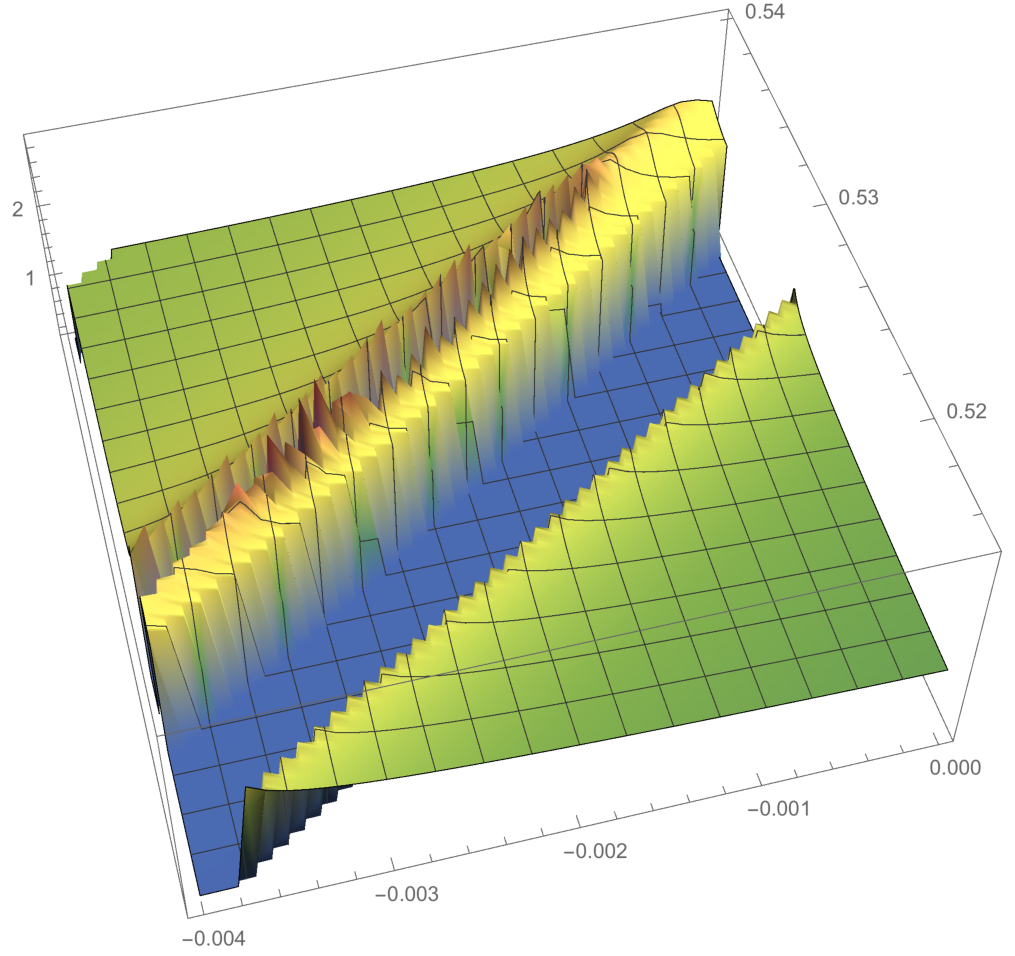
\includegraphics[scale=0.5]{Immagini/spiked3N2-zoomed.pdf}
\caption{A zoom of the region of the domain of $\bar \rho$ where the peaks are located.}
\label{fig:5}
\end{center}
\end{figure}






\newpage 
\subsection{Polynomial Analysis}
A valuable tool can be the analysis of the solutions expanded in power series around the origin or around a non trivial vacuum.
The expansion around the origin in case of a broken phase provides typically a slightly worst description with respect to the second one, which is in general preferable.

In a neighborhood of the origin  the  polynomial expansions of $u(\rho)$ and $f(\rho)$ are:
\begin{equation}
 u(\rho) = \sum _{n=2}^{N_u} \frac{\lambda _n \rho^n}{n!}+\lambda _0
\end{equation}\begin{equation}
 f(\rho) = \sum _{n=0}^{N_f} \frac{f_n \rho^n}{n!}
\end{equation}
and, in the neighborhood of the potential minimum:
\begin{equation}
 u(\rho) = \sum _{n=2}^{N_u} \frac{\lambda _n (\rho -\kappa )^n}{n!}+\lambda _0
\end{equation}\begin{equation}
 f(\rho) = \sum _{n=0}^{N_f} \frac{f_n (\rho -\kappa )^n}{n!}
\end{equation}
Where I have defined $\kappa$ as the value of the dimensionless field modulus square at the minimum of the potential:
\begin{equation}
u'(\kappa) = 0
\end{equation}


Substituting these polynomial expansions of a given order into the fixed point equations and expanding around zero or around the minimum, on obtains a set of algebraic equations whose solutions may give an approximate 
polynomial solution to the differential equation within some bounded region.
Typically one finds many spurious solutions and it is a difficult task to search for a ``good'' one. Nevertheless, if one succeed in this, very often one obtains locally a pretty good approximation of the solution.

We show here an exampe of a polynomial solution obtained with a expansion around a non trivial vacuum for the case $N=1.5$ in Tab.\ref{tab:poli}.

\begin{figure}
\begin{center}
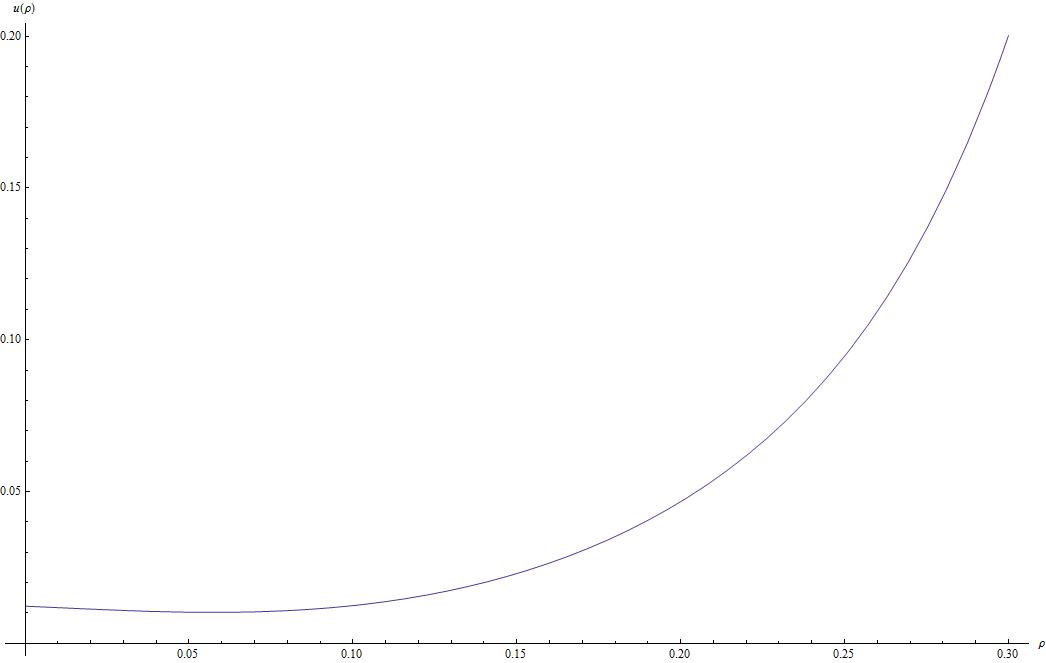
\includegraphics[scale=0.25]{Immagini/plotuN1.jpg}
\caption{Plot of the polynomial expansion around the nontrivial minimum of the dimensionless effective potential $u(\rho)$ for N=3/2.}
\label{fig:plotfN1}
\end{center}
\end{figure}

\begin{table}
  \begin{center}
    \begin{small}
      \begin{tabular}{|c|c|}
 \hline 
 &   \textbf{Results of the polynomial analysis for $N=3/2$, $N_u = 7$ and $N_f = 6$} \\ \hline 
$\lambda_0$ & $0.010174597$  \\ \hline
$\kappa$ & $0.057469286$ \\ \hline 
$\lambda_2$ & $1.9926498$ \\ \hline 
$\lambda_3$ & $34.887704$ \\ \hline 
$\lambda_4$ & $-236.78017$ \\ \hline 
$\lambda_5$ & $8412.4279$ \\ \hline 
$\lambda_6$ &  $-257655.64$ \\ \hline 
$\lambda_7$ &  $9.8750075*10^6$\\ \hline 
$f_0$ & $  0.082295013$ \\ \hline 
$f_1$ & $0.31782706$ \\ \hline 
$f_2$ & $  -0.76423349$ \\ \hline 
$f_3$ & $12.391789$ \\ \hline 
$f_4$ & $-203.83313$ \\ \hline 
$f_5$ & $3149.2212$ \\ \hline 
$f_6$ & $-74077.151$ \\ \hline 

\end{tabular}
    \end{small}
  \end{center}
\caption{Numerically evaluated coefficients $\lambda_i$ and $f_i$ for $N_u = 7$ and $N_f=6$ for the expansion of the potential around the non trivial minimum, in the case $N=3/2$.}
\label{tab:poli}
\end{table}



\begin{figure}
\begin{center}
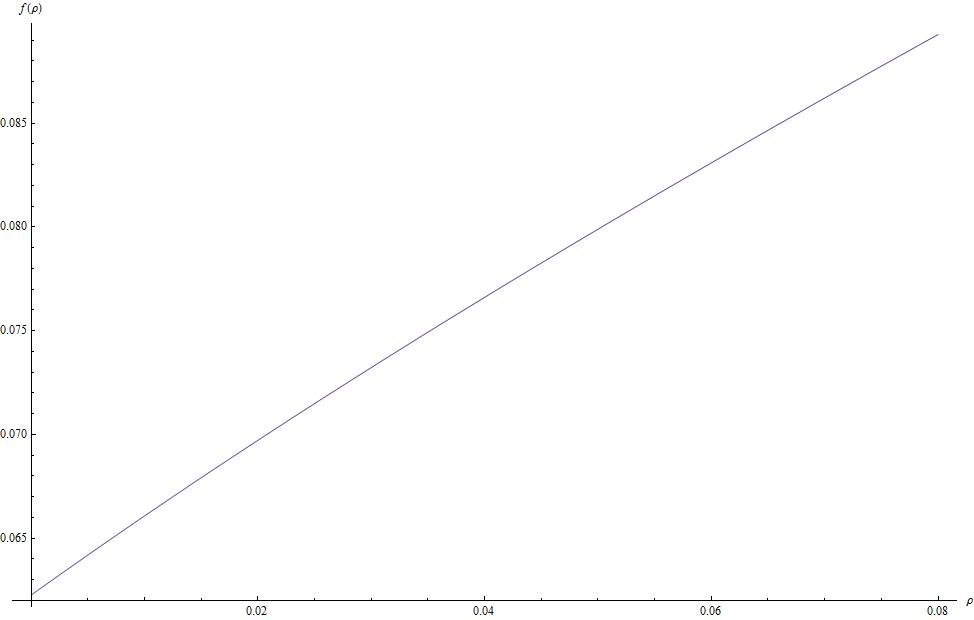
\includegraphics[scale=0.25]{Immagini/plotfN1.jpg}
\caption{Plot of the polynomial expansion of $f(\rho)$  around the non trivial minimum of  the potential for N=3/2.}
\label{fig:plotfN1}
\end{center}
\end{figure}








